\documentclass[a4paper,11pt,fleqn]{article}%fleqn pour aligner les equations à gauche
\usepackage{../.../Styles/Cours}


\newcommand{\chnum}{Chapitre 1}
\newcommand{\chtitle}{Identification d'espèces chimiques}
\newcommand{\dtype}{Cours}


\begin{document}
\maketitle

\section{Définitions}
	\subsection{Corps purs}
La matière est constituée d'entités chimiques (molécules, atomes, ions). Une espèce chimique est un ensemble d'entités chimiques identiques. Un corps pur est constitué d'une seule espèce chimique. un mélange est constitué de plusieurs espèces chimiques.\\
À température et pression ambiante un sorps pur peut être :
\begin{itemize*}
	\item à l'état solide : l'or \ce{Au(s)}, le chlorure de sodium \ce{NaCl(s)}
	\item à l'état liquide : l'eau \ce{H2O(l)}, l'acétone \ce{C3H6O(l)}
	\item à l'état gazeux : l'hélium \ce{He(g)}, le dioxygène \ce{O2(g)}
\end{itemize*}

	\subsection{Mélanges}
Un mélange est composé d’au moins deux espèces chimiques. La composition d’un mélange est
donnée par le pourcentage massique ou volumique de chaque espèce dans le mélange.\\

\textit{Exemple : le pourcentage massique de cuivre Cu(s) dans une pièce de 10 centimes d’euros de
masse $m$ = \SI{4,14}{g}, est de \SI{89}{\percent}. Quelle masse de cuivre contient-elle ?}

\begin{itemize}
	\item Dans un mélange homogène on ne distingue aucun constituant à l’œil nu.\\
ex : une solution non saturée est un mélange homogène, l’air est un mélange homogène de
plusieurs gaz …
	\item Dans un mélange hétérogène on distingue au moins 2 constituants à l’œil nu.\\
ex : eau et huile, eau et cuivre, une solution saturée …
\end{itemize}

\section{Identification d'espèces chimiques}
	\subsection{par des tests physiques}
Chaque espèce chimique a son propre ensemble de caractéristiques physiques permettant de
l’identifier.
		\subsubsection{la masse volumique (Voir TP 1 - Partie 1)}
La masse volumique d’une espèce chimique est égale au quotient de la masse de l’espèce par
son volume :\\
\begin{tabular}{>{\centering}m{6cm}|m{13cm}}
	\multirow{3}{*}{$\rho = \dfrac{m}{V}$} & avec $m$ en grammes\\
	& $V$ en litre\\
	& $\rho$ en \unit{\gram\per\liter}\\
\end{tabular}
La masse volumique de l’eau est égale à \SI{1000}{\gram\per\liter}. Il suffit donc de mesurer la masse et le volume d’une espèce chimique pour en déterminer la masse volumique et pouvoir l’identifier.
		\subsubsection{la température de changement d'état}
Le changement d’état d’un corps pur se fait à température constante pour une pression donnée.
Pour identifier une espèce on peut mesurer sa température de fusion $\theta_f$ pour un solide ou sa température d’ébullition $\theta_{eb}$ avec un thermomètre.
	\subsection{par des tests chimiques (Voir TP 1 - Partie 2)}
	Le test chimique est une expérience dont le résultat (changement de couleur, précipité …) permet
de mettre en évidence la présence de certaines espèces chimiques (molécules ou ions en solution
aqueuse).
\begin{table}[h!]
	\caption*{Exemples de tests chimiques}
	\begin{tabular}{|>{\centering}m{.2\linewidth}|>{\centering}m{.2\linewidth}|>{\centering}m{.3\linewidth}|>{\centering\arraybackslash}m{.2\linewidth}|}
	\hline
	\textbf{Exepèce chimique à identifier} & \textbf{Test} & \textbf{Schéma de l'expérience} & \textbf{Résultat positif}\\
	\hline
	Eau (liquide) & Sulfate de cuivre anhydre (solide blanc) & 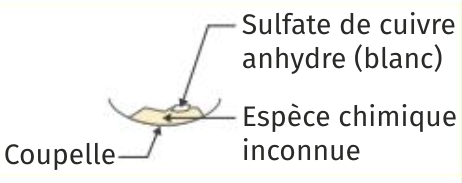
\includegraphics[width=\linewidth]{Ressources/2GT_C01_Cours_Fig1.png}& Le sulfate de cuivre anhydre devient bleu.\\
	\hline
	Dioxyde de carbone & Eau de chaux & 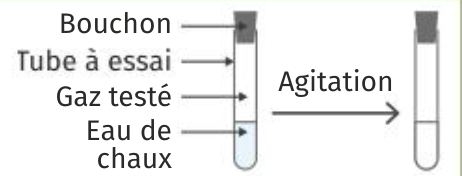
\includegraphics[width=\linewidth]{Ressources/2GT_C01_Cours_Fig2.png}& L'eau de chaux se trouble.\\
	\hline
	Ions chlorure & Solution de nitrate d'argent & 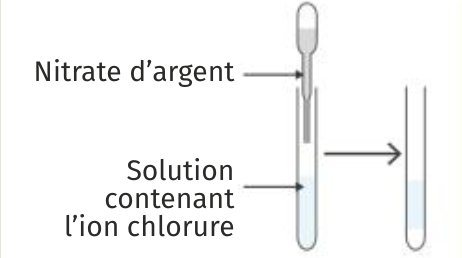
\includegraphics[width=\linewidth]{Ressources/2GT_C01_Cours_Fig3.png}& Il se forme un précipité blanc. \\
	\hline
	\end{tabular}
\end{table}
	\subsection{Par chromatographie sur couche mince}
La chromatographie sur couche mince permet d’identifier certaines espèces chimiques d’un
mélange homogène. Elle se base sur la différence d’affinité des espèces chimiques entre deux
phases : une phase mobile (éluant) et une phase fixe (support).\\
L’identification des espèces chimiques se fait par comparaison avec des espèces pures servant
de référence.
\begin{figure}[h!]
	\centering
	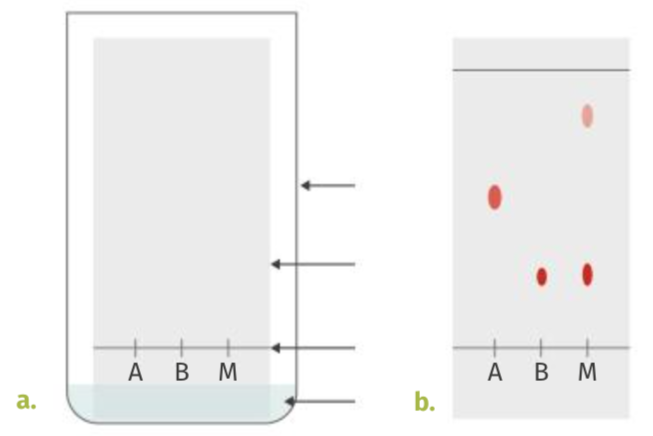
\includegraphics[width=.4\linewidth]{Ressources/2GT_C01_Cours_Fig4.png}
\end{figure}
\end{document}
